% Options here are passed to the article class.
% Most common options: 10pt, 11pt, 12pt
\documentclass[10pt]{datasheet}

% Input encoding and typographical rules for English language
\usepackage[utf8]{inputenc}
\usepackage[english]{babel}
\usepackage[english]{isodate}

% tikz is used to draw images in this example, but you can
% also use \includegraphics{}.
\usepackage{graphicx}

% These define global texts that are used in headers and titles.
\title{TP01: Decimal Encoded Variable Instant Dropperline}
\author{Andrews54757}
\tags{transport, decimal-encoded}
\date{21 December 2022}
\revision{Revision 1}
\begin{document}
\maketitle

\section{Features}

\begin{itemize}
\item{Constant time insertion}
\item{10gt throughput}
\item{Fired twice for overflow handling}
\end{itemize}

\section{Applications}

\begin{itemize}
\item{Item transportation for halls.}
\end{itemize}

\section{General Description}
Takes two comparator inputs (one decimal, one half-decimal) and deposits items in the decoded slice in constant time. The dropperline is fired twice per insertion to clear any potential overflow items. 10gt-able.

\vfill\break

\begin{figure}[h]
    \centering
    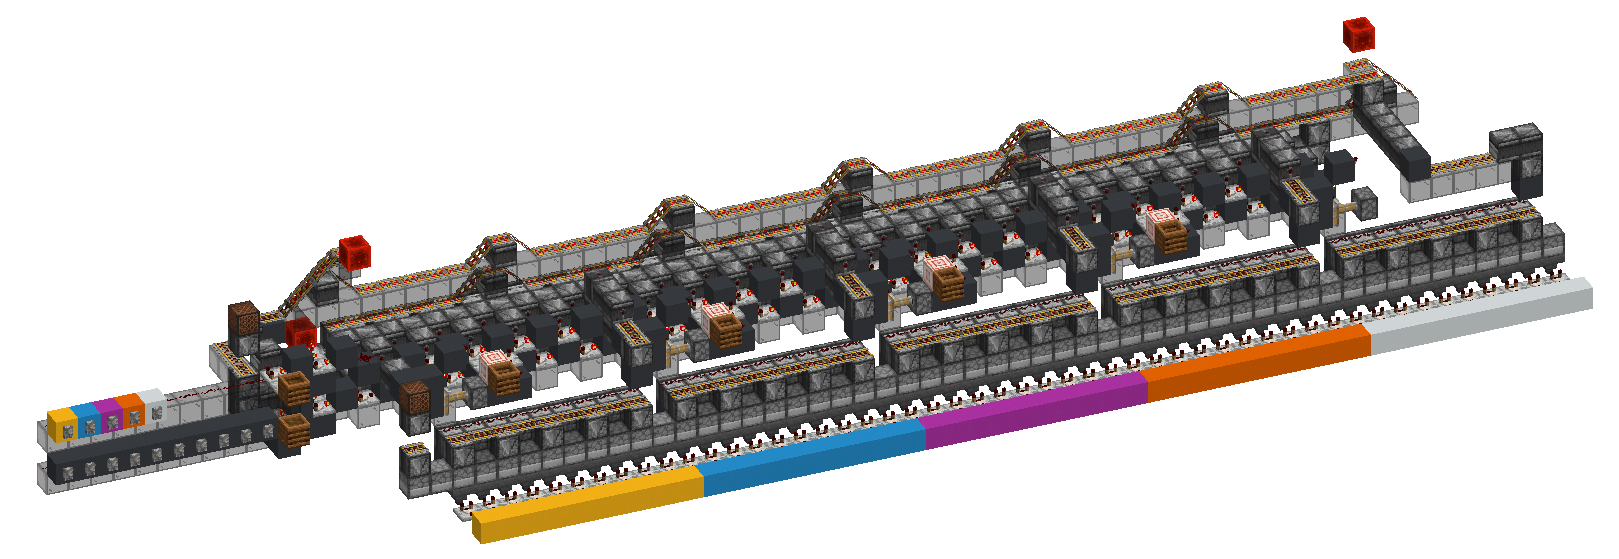
\includegraphics[width=0.48\textwidth]{vardrop2.png}
    \caption{\centering Decimal Encoded Variable Instant Dropperline}
\end{figure}

% For wide tables, a single column layout is better. It can be switched
% page-by-page.
\onecolumn

\section{Device Specifications}

\begin{table}[h]
    \caption{Inputs}
    \begin{tabularx}{\textwidth}{l | c | X}
        \thickhline
        \textbf{Name} & \textbf{Range} & \textbf{Description} \\
        \hline
        HDigit 1 & 1-5 & Half-digit indicates section \\
        \hline
        Digit 2 & 1-10 & Digit indicates slice. \\
        \hline
        Item input & Item & Item to be moved. \\
        \hline
        Clock signal & Pulse & Executes order. \\
        \thickhline
\end{tabularx}
\end{table}

\begin{table}[h]
    \caption{Outputs}
    \begin{tabularx}{\textwidth}{l | c | X}
        \thickhline
        \textbf{Name} & \textbf{Range} & \textbf{Description} \\
        \hline
        Outputs & Item & Outputs item to one of fifty slices corresponding to code. \\
        \hline
        Overflow Output & Item & Outputs overflow items at end. \\
        \thickhline
\end{tabularx}
\end{table}

\begin{table}[h]
    \caption{Device Specifications}
    \begin{tabularx}{\textwidth}{l | c c c | c | X}
        \thickhline
        \textbf{Parameter} & \textbf{Min.} & \textbf{Typ.} & \textbf{Max.} &
        \textbf{Unit} & \textbf{Conditions} \\
        \hline
        Throughput  & 10 & - & - & gt & Normal Usage \\
        \hline
        MC Version & 1.16 & 1.17.1 & - & MCV & Latest version at time of writing: 1.19.3\\
        \hline
        Dimensions & & 67 x 11 x 10 & & Blocks & \\
        \thickhline
\end{tabularx}
\end{table}
\newpage
\section{Testing Data}
\begin{table}[h]
\caption{Executed Tests}
\begin{tabularx}{\textwidth}{l | X}
    \thickhline
    \textbf{Test} & \textbf{Result} \\
    \hline
    Decoding test & Device was able to decode with 10gt clocked input. \\
    \thickhline
\end{tabularx}
\end{table}

\section{Download Information}
\begin{table}[h]
    \caption{Download Information}
    \begin{tabularx}{\textwidth}{l | l | l | X}
        \thickhline
        \textbf{Identifier} & \textbf{MC} & \textbf{File} & \textbf{Description} \\
        \hline
        TP01 & 1.17.1 & TP01\_Decimal\_Encoded\_Variable\_Instant\_Dropperline.litematic & Schematic of device. \\
        \hline
        \thickhline
    \end{tabularx}
\end{table}

\end{document}

